%%%%%%%%%%%%%%%%%%%%%%%%%%%%%%%%%%%%%%%%%
% a0poster Portrait Poster
% LaTeX Template
% Version 1.0 (22/06/13)
%
% The a0poster class was created by:
% Gerlinde Kettl and Matthias Weiser (tex@kettl.de)
% 
% This template has been downloaded from:
% http://www.LaTeXTemplates.com
%
% License:
% CC BY-NC-SA 3.0 (http://creativecommons.org/licenses/by-nc-sa/3.0/)
%
%%%%%%%%%%%%%%%%%%%%%%%%%%%%%%%%%%%%%%%%%

%----------------------------------------------------------------------------------------
%	PACKAGES AND OTHER DOCUMENT CONFIGURATIONS
%----------------------------------------------------------------------------------------

\documentclass[a0,portrait]{a0poster}

\usepackage{multicol} % This is so we can have multiple columns of text side-by-side
\columnsep=100pt % This is the amount of white space between the columns in the poster
\columnseprule=3pt % This is the thickness of the black line between the columns in the poster

\usepackage[svgnames]{xcolor} % Specify colors by their 'svgnames', for a full list of all colors available see here: http://www.latextemplates.com/svgnames-colors

\usepackage{times} % Use the times font
%\usepackage{palatino} % Uncomment to use the Palatino font

\usepackage{graphicx} % Required for including images
\graphicspath{{figures/}} % Location of the graphics files
\usepackage{booktabs} % Top and bottom rules for table
\usepackage[font=small,labelfont=bf]{caption} % Required for specifying captions to tables and figures
\usepackage{amsfonts, amsmath, amsthm, amssymb} % For math fonts, symbols and environments
\usepackage{wrapfig} % Allows wrapping text around tables and figures
\usepackage[french]{babel}
\usepackage[utf8]{inputenc}
\begin{document}

%----------------------------------------------------------------------------------------
%	POSTER HEADER 
%----------------------------------------------------------------------------------------

% The header is divided into two boxes:
% The first is 75% wide and houses the title, subtitle, names, university/organization and contact information
% The second is 25% wide and houses a logo for your university/organization or a photo of you
% The widths of these boxes can be easily edited to accommodate your content as you see fit

\begin{minipage}[b]{0.75\linewidth}
\veryHuge \color{NavyBlue} \textbf{Les transformées temps-fréquence appliquées au Non-Intrusive Load Monitoring} \color{Black}\\ % Title
\Huge\textit{Détection, identification et classification des charges électriques}\\[2cm] % Subtitle
\huge \textbf{Mahfoud Drouaz, Ali Moukadem, Bruno Colicchio, Alain Dienterlein \& Djaffar Ould-Abdeslam}\\[0.5cm] % Author(s)
\huge Université de Haute-Alsace, 61 rue Albert Camus 68093 Mulhouse\\[0.4cm] % University/organization
\Large \texttt{Mahfoud.drouaz@uha.fr}\\

\includegraphics[width=15cm]{UHA.pdf}
\includegraphics[width=15cm]{MIPS.pdf}
\end{minipage}
%
\begin{minipage}[b]{0.25\linewidth}

\includegraphics[width=15cm]{JNRDM.png}\\


\end{minipage}

\vspace{1cm} % A bit of extra whitespace between the header and poster content

%----------------------------------------------------------------------------------------

\begin{multicols}{2} % This is how many columns your poster will be broken into, a portrait poster is generally split into 2 columns

%----------------------------------------------------------------------------------------
%	ABSTRACT
%----------------------------------------------------------------------------------------

\color{Navy} % Navy color for the abstract

\begin{abstract}

Ce résumé présente les travaux de thèse qui s'inscrivent dans le cadre de l'identification non-intrusive des charges électriques connu aussi sous le nom de NILM (Non-intrusive Load Monitoring). Il présente l'application des transformées temps-fréquence à l'analyse des transitoires de mise en marche des appareils électriques. Cette analyse permet d'extraire les signatures de ces transitoires dans le but de caractériser et faciliter l'identification et le suivi de consommation énergétique des charges électriques.

\end{abstract}

%----------------------------------------------------------------------------------------
%	INTRODUCTION
%----------------------------------------------------------------------------------------

\color{SaddleBrown} % SaddleBrown color for the introduction

\section*{Introduction}

Dans le contexte d'une maîtrise de la consommation énergétique des foyers, une connaissance détaillée de la consommation individuelle des équipements électriques est nécessaire et importante. Depuis les travaux pionniers de Hart en 1992 \cite{hart1992} sur le NILM (Non-Intrusive Load Monitoring), l'intérêt de cette méthode a trouvé une place au sein de la communauté scientifique et industrielle. Le NILM s’attache à obtenir des informations de manière non-intrusive à partir d'un seul point de mesure, étudier la désagrégation des courbes de charges afin d'identifier les appareils connectés sur le réseau électrique et ainsi réaliser le suivi leurs consommations. La reconnaissance des charges s’appuie sur l’extraction de signatures électriques que les appareils émettent lors de leur fonctionnement. Les premiers modèles d’identification dans le NILM consistaient à extraire des descripteurs à partir du régime établi, tels que le courant efficace, la puissance, le taux d’harmoniques émis par les appareils, etc. De nos jours, de nombreux travaux visent à étudier le régime transitoire \cite{naitmeziane2016, sanquer2013}, afin d'apporter plus de performances à l'identification et la classification des charges électriques. Le régime transitoire étudie l'instant de mise en marche d'une charge électrique. Pour ce faire, nous exploitons les outils de traitement du signal temps-fréquence. Les transformées temps-fréquence permettent d'étudier l'évolution fréquentielle d'un signal dans le temps, dans le cadre des travaux réalisés dans cette thèse, elles nous permettent d'extraire les caractéristiques du transitoire de mise en marche associées à chaque charge électrique. Durant cette thèse, une plateforme d'acquisition et de simulation de scénarios a été développée. Une base de données de mesures a été par la suite réalisée sur plusieurs types d'appareils électriques afin de pouvoir tester nos algorithmes de classification. Enfin, l'application des transformées temps-fréquence à l'analyse des transitoires de mise en marche des charges électriques offre une nouvelle voie pour l'application de ces outils d'analyse.

%----------------------------------------------------------------------------------------
%	OBJECTIVES
%----------------------------------------------------------------------------------------

\color{DarkSlateGray} % DarkSlateGray color for the rest of the content

\section*{Main Objectives}

\begin{enumerate}
\item 
\end{enumerate}

%----------------------------------------------------------------------------------------
%	MATERIALS AND METHODS
%----------------------------------------------------------------------------------------

\section*{Matériels and Méthodes}
Le système de mesure a été développé au seins de notre laboratoire, afin de permettre la réalisation de mesures réelles sur des appareils électriques. Il est compose de :
\begin{enumerate}
\item Une carte composée de 9 capteurs de courants à effet Hall.
\item Une sonde différentielle pour la mesure de la tension électrique.
\item Des cartes d'acquisition de données labjack U3-HV et U6.
\item Une carte de traitement de données PYNQ-Z1.
\item Plusieurs charges électriques pour simuler des scénarios.
\end{enumerate}

\begin{center}\vspace{1cm}
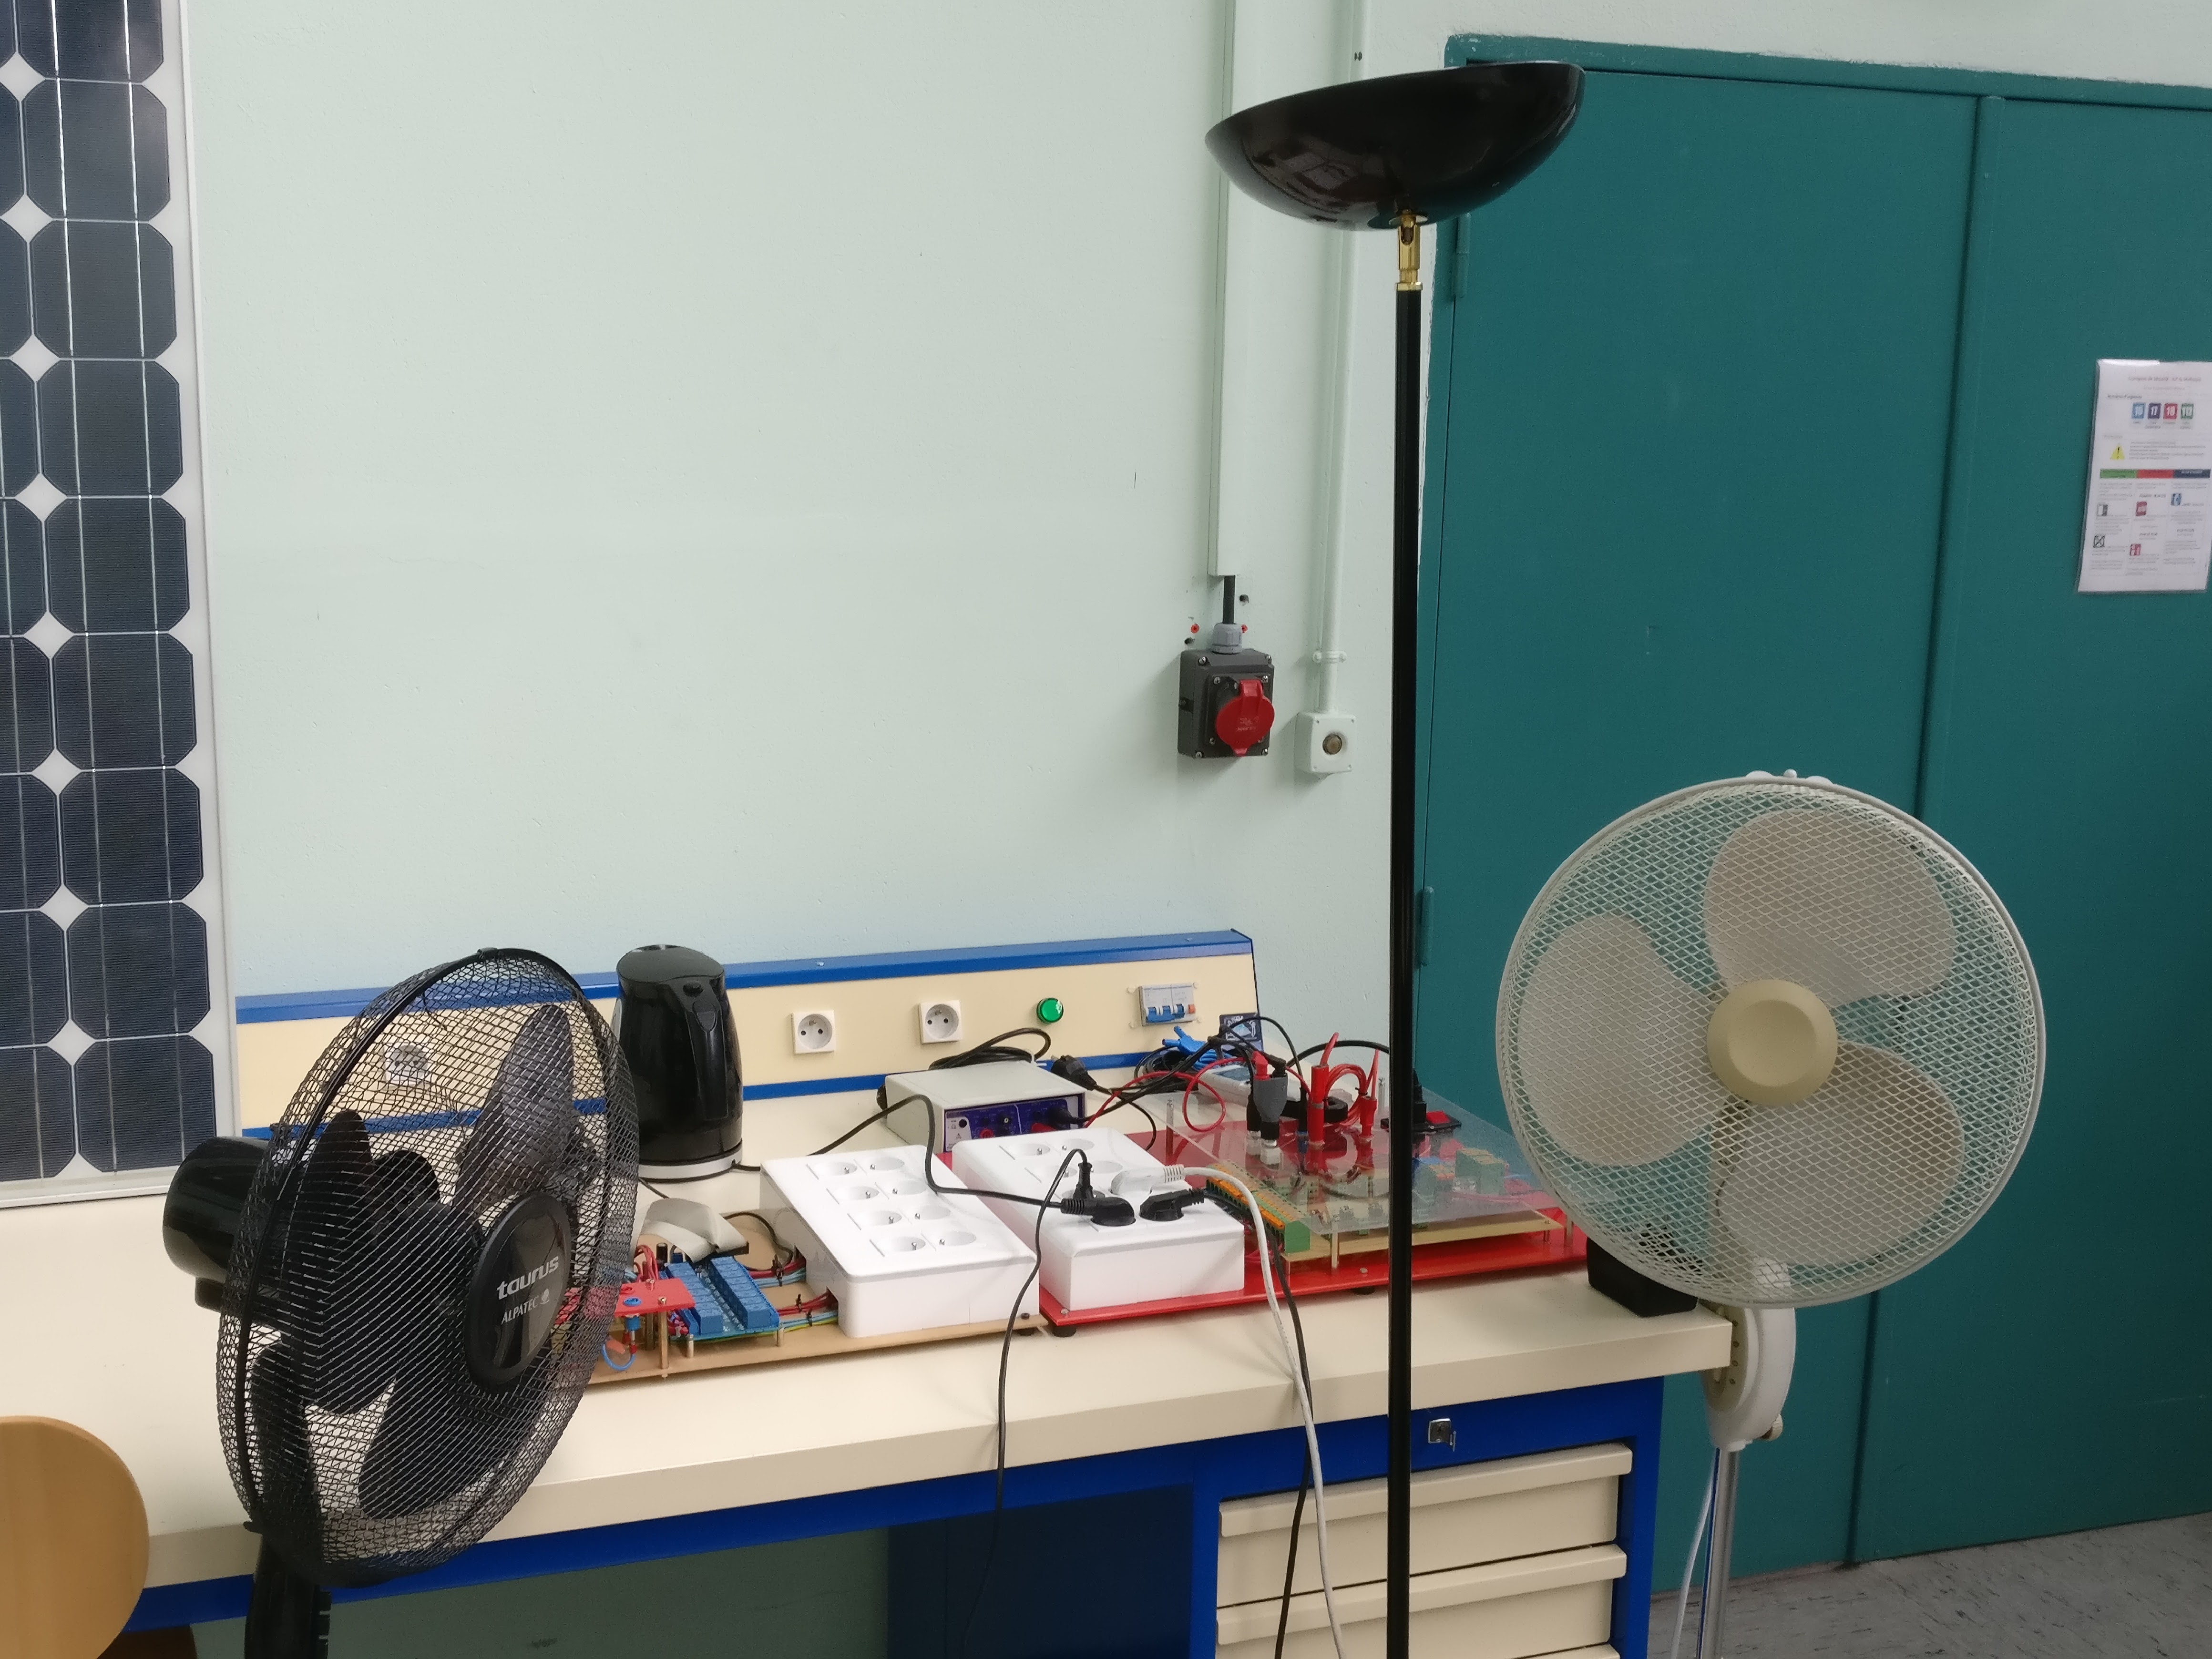
\includegraphics[width=1\linewidth]{systeme_mesure.jpg}
\captionof{figure}{\color{Green} Figure caption}
\end{center}\vspace{1cm}

%------------------------------------------------

\subsection*{Outils Mathématiques}

La transformée de Stockwell \cite{stockwell1996localization}
 d'un signal $x(t)$ est définie comme suit :
\begin{equation*}
	ST_{x}(\tau,f) = \int_{-\infty}^{+\infty} x(t) w(\tau-t,f) e^{-2\textit{i}\pi ft} \, \mathrm{d}t
	\label{eq.3}
\end{equation*}
Elle permet d'améliorer la résolution fréquentielle dans les basses fréquences et la résolution temporelle dans les hautes fréquences.\\
La fenêtre Gaussienne $w$ est une fonction du temps est de la fréquence, elle est choisie tel que:
\begin{equation*}
	w(t, f) = \frac{1}{\sigma(f) \sqrt{2 \pi}} e^{{-t^2}/{2\sigma(f)^2}}
	\label{eq.4}
\end{equation*}
La transformée de Stockwell est dite une transformée multi-résolution, ou la largeur de la fenêtre $\sigma$ est une fonction de la fréquence est définie comme suit :
\begin{equation*}
	\sigma(f) = \frac{1}{|f|}
	\label{eq.5}
\end{equation*}
\begin{equation*}
	w(t,f) = \frac{|f|}{\sqrt{2 \pi}} e^{{-f^{2}t^{2}}/{2}}
	\label{eq.6}
\end{equation*}
Pour assurer la réversibilité de la transformée de Stockwell, la fenêtre Gausienne est normalisée tel que :
\begin{equation*}
	\int_{-\infty}^{+\infty} w(t,f) \, \mathrm{d}t = 1
	\label{eq.7}
\end{equation*}

%----------------------------------------------------------------------------------------
%	RESULTS 
%----------------------------------------------------------------------------------------

\section*{Résultats}


%----------------------------------------------------------------------------------------
%	CONCLUSIONS
%----------------------------------------------------------------------------------------

\color{SaddleBrown} % SaddleBrown color for the conclusions to make them stand out

\section*{Conclusions}

\begin{itemize}
\item Développement d'une carte d'acquisition et d'une maquette simulations de charges électriques.
\item Constitution d'une base de données de transitoires individuels et scénarios de différents types de charges électriques.
\item Application des transformées temps-fréquences pour la caractérisation des transitoires de mise en marche.
\item Développement d'algorithme pour du traitement en ligne et temps-réels.
\end{itemize}

\color{DarkSlateGray} % Set the color back to DarkSlateGray for the rest of the content

%----------------------------------------------------------------------------------------
%	FORTHCOMING RESEARCH
%----------------------------------------------------------------------------------------

\section*{Forthcoming Research}

%----------------------------------------------------------------------------------------
%	REFERENCES
%----------------------------------------------------------------------------------------

%\nocite{*} % Print all references regardless of whether they were cited in the poster or not
\bibliographystyle{plain} % Plain referencing style
\bibliography{sample} % Use the example bibliography file sample.bib

%----------------------------------------------------------------------------------------
%	ACKNOWLEDGEMENTS
%----------------------------------------------------------------------------------------

\section*{Acknowledgements}

%----------------------------------------------------------------------------------------

\end{multicols}
\end{document}